\documentclass{article}
\usepackage[utf8]{inputenc}
\usepackage{amsmath}
\usepackage{multirow}
\usepackage[inline]{enumitem}
\usepackage{graphicx}
\graphicspath{ {./images/} }
\newcommand{\lt}{\latintext}
\newcommand{\gt}{\greektext}
\usepackage{tikz}
\usepackage{pgfplots}
\usepackage{hyperref}

\pgfplotsset{compat = newest}

\title{\gt \textbf{Δεύτερη Υποχρεωτική Εργασία}}
\author{\gt \LargeΟνοματεπώνυμο: Ασημάκης Κύδρος \\ ΑΕΜ: 3881}
\date{\gt \Large26 Ιανουαρίου 2022}

%%Activate Greek ASCII characters
\usepackage[english,greek]{babel}

\begin{document}
\maketitle

\pagebreak
%%------------ΠΕΜΠΤΗ ΑΣΚΗΣΗ------------%%
\section{\gt Πέμπτη Άσκηση}
\Large
\gt Για την προσέγγιση του ημιτόνου, χρησιμοποιήθηκαν τα \\εξής σημεία-δείγματα:
\begin{center}
    \begin{tabular}{|c|c|}
        \hline
        \lt x (radians)    & \lt sin(x)    \\\hline
        $-\pi$             & 0         \\\hline
        $\frac{-\pi}{2}$   & -1        \\\hline
        $\frac{-\pi}{4}$   & -0.707106 \\\hline
        $\frac{-\pi}{8}$   & -0.382683 \\\hline
        0                  & 0           \\\hline
        1                  & 0.841470    \\\hline
        $\frac{\pi}{8}$    & 0.382683  \\\hline
        $\frac{\pi}{4}$    & 0.707106  \\\hline
        $\frac{\pi}{2}$    & 1         \\\hline
        $\pi$              & 0         \\\hline
    \end{tabular}
\end{center}
\gt (με την ακρίβεια που φαίνεται).\\

\textbf{\gt α) Μέθοδος \lt Lagrange}\\
\gt Στην πρώτη εκτέλεση, ο αλγόριθμος καλεί τα σημεία και τα αποθηκεύει στην μνήμη
\gt για να μην καλούνται συνεχώς. Έπειτα χτίζει τον γνωστό τύπο:
\begin{equation*}
    L_i(x) = \displaystyle \prod_{j=0, i \neq j}^{n}\frac{x - x_j}{x_i - x_j}
\end{equation*}
\gt θεωρώντας όπου \lt x \gt την παράμετρο της συνάρτησης και ενημερώνει την (αρχικά 0) σούμα:
\begin{equation*}
    sum += y_iL_i(x)
\end{equation*}
\gt Έφοσον χρησιμοποιούμε κατευθείαν την ζητούμενη τιμή στην κατασκευή του πολυωνύμου,
\gt η σούμα αυτή αντιπροσωπεύει το αποτέλεσμα-προσέγγιση του ημιτόνου για την περασμένη τιμή.

\textbf{\gt β) Μέθοδος \lt splines\gt (φυσικά κυβικά)}\\
\gt Θεωρώντας κάθε \lt spline \gt ως πολυώνυμο της μορφής
\begin{equation*}
    y = a + b(x - x_0) + c(x - x_0)^2 + d(x - x_0)^3
\end{equation*}
\gt Ορίζουμε την πεντάδα \lt(a, b, c, d, $x_0$) \gt που θα αντιπροσωπεύει ένα \lt spline.
\gt Αφού η θεωρητική μεθοδολογία απαιτεί αόριστη ολοκλήρωση, βρίσκουμε τα \lt splines
\gt για τα σημεία μας μέσω του \href{https://en.wikipedia.org/wiki/Spline_(mathematics)}{\textbf{\gt εξής αλγορίθμου}}.

\gt Έχοντας βρει τα \lt splines, \gt η συνάρτηση-προσέγγιση τα αποθηκεύει στην μνήμη για να μην
\gt καλούνται συνεχώς. Καλεί με τον ίδιο τρόπο και τα ίδια τα σημεία για να τα χρησιμοποιήσει ως 
\gt πεδία ορισμού των \lt splines. \gt Για κάθε παράμετρο, βρίσκει σε πιο πεδίο ορισμού ανήκει και
\gt επιστρέφει το αποτέλεσμα του αντίστοιχου \lt spline \gt για την συγκεκριμένη παράμετρο.

\textbf{\gt γ) Μέθοδος ελαχίστων τετραγώνων}\\
\gt Η συνάρτηση δέχεται ως ορίσματα το σημείο \lt x \gt για το οποίο ζητείται η τιμή του,
\gt καθώς και ο βαθμός του πολυωνύμου-προσέγγιση που απαιτείται. Στην προκειμένη περίπτωση
\gt χρησιμοποιήθηκε τρίτου βαθμού πολυώνυμο.

\gt Αρχικά η συνάρτηση καλεί τους συντελεστές του πολυωνύμου για να τους αποθηκεύεσει στην
\gt μνήμη ώστε να μην καλούνται συνεχώς. Αυτή η διαδικασία καλεί τα σημεία-δείγματα και αρχικοποιεί
\gt με αυτά τους πίνακες \lt A, b:
\begin{equation*}
    \textbf{A} = 
    \begin{bmatrix}
         1 & x_{i} & x_{i}^2 & x_{i}^3\\
         .& . & . & .
    \end{bmatrix}
\end{equation*}
\begin{equation*}
    \textbf{b} = 
    \begin{bmatrix}
         y_i\\
         ...
    \end{bmatrix}
\end{equation*}
$ i = 0, 1, ..., n - 1 $ \quad n = \gt αριθμός σημείων. 
\gt Μετέπειτα υπολογίζει τους πίνακες \lt $A^{T}A$, $A^{T}b$ \gt χρησιμοποιώντας τις μεθόδους
\gt και τις κλάσεις των προηγούμενων ασκήσεων. Η λύση του
\begin{equation*}
    (A^{T}A)c = A^{T}b
\end{equation*} 
\gt μέσω \lt Gauss \gt περιγράφει τους συντελεστές.

\gt Έχοντας κάνει αυτά, η συνάρτηση-προσέγγιση επιστρέφει την τιμή
\begin{equation*}
    c_0 + c_1x + c_2x^2 + c_3x^3 
\end{equation*}
\gt για κάθε παράμετρο \lt x.

\gt Τρέχουμε τις παραπάνω προσομοιώσεις για διακόσιες τυχαίες τιμές στο $[-\pi,\pi]$. 
\gt Προβάλλοντας τις αποκλίσεις τους για κάθε μέθοδο σε διάγραμμα, βλέπουμε το εξής:
\begin{center}
    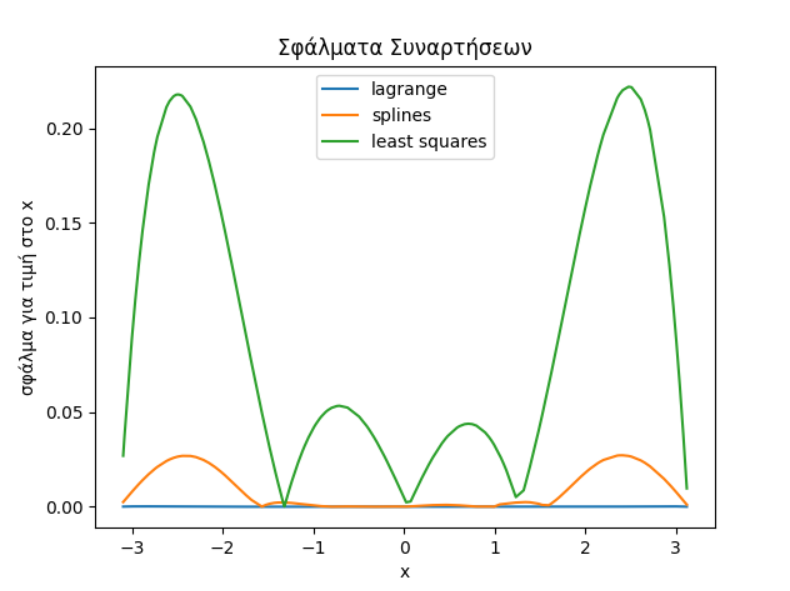
\includegraphics[scale=0.7]{images/res_graph.png}
\end{center}
\gt Παρατηρούμε ότι, από άποψη ελαχιστοποίησης σφάλματος, η \lt lagrange \gt είναι κατά πολύ η
\gt καλύτερη μέθοδος. Ακολουθεί η \lt splines \gt και τελευταία είναι η ελάχιστων τετραγώνων, με 
\gt μεγάλο σφάλμα, κάτι αναμενόμενο, καθώς από την φύση του το πολυώνυμο που παράγει δεν περνάει από
\gt κανένα από τα δωσμένα σημεία.

\gt Συγκρίνοντας τα αποτελέσματα, μπορούμε να πούμε ότι η μέθοδος \lt lagrange \gt πετυγχαίνει
\gt τουλάχιστον 3 δεκαδικά ψηφία ακρίβειας, η μέθοδος των \lt splines \gt πετυγχαίνει τουλάχιστον
\gt 1 και τα ελάχιστα τετράγωνα το πολύ 2.

\pagebreak
%%------------ΈΚΤΗ ΑΣΚΗΣΗ------------%%
\section{\gt Έκτη Άσκηση}

\gt Καλούμαστε να βρούμε προσεγγιστικά την τιμή του
\begin{equation*}
    I = \int_{0}^{\frac{\pi}{2}}sin(x)dx
\end{equation*}
\gt Προτού αρχίσουμε την προσεγγιστική διαδικασία, λύνουμε χειροκίνητα το ολοκλήρωμα για να
\gt βρούμε ότι η πραγματική τιμή του είναι 1, κάτι που θα χρησιμεύσει αργότερα.

\gt Τόσο η μέθοδος τραπεζίου όσο και του \lt Simpson \gt απαιτούν ομοιόμορφη κατανομή του πεδίου
\gt ορισμού. Μέσω της συνάρτησης \lt divide\textunderscore domain\textunderscore equal(),
\gt χωρίζουμε το $[0, \frac{\pi}{2}]$ σε 10 ίσα τμήματα. Δηλαδή τα 11 σημεία είναι:
\begin{center}
    $\begin{bmatrix}
        0              \\
        \frac{\pi}{20} \\
        \frac{\pi}{10} \\
        \frac{3\pi}{20}\\
        \frac{\pi}{5}  \\
        \frac{\pi}{4}  \\
        \frac{6\pi}{20}\\
        \frac{7\pi}{20}\\
        \frac{2\pi}{5} \\
        \frac{9\pi}{20}\\
        \frac{\pi}{2}  \\
    \end{bmatrix}$
\end{center}

\textbf{\gt α) Μέθοδος τραπεζίου}\\
\gt Η συνάρτηση δέχεται ως παραμέτρους το πεδίο ορισμού και τον αριθμό των σημείων.
\gt Διαχωρίζει το πεδίο με τον προαναφερώμενο τρόπο και, με τα 11 σημεία που πήρε,
\gt εκτελεί την γνωστή πράξη:
\begin{equation*}
    I = \frac{b - a}{2N}(f(x_0) + f(x_N) + 2\sum_{i=1}^{N-1}f(x_i))
\end{equation*}
\gt για \lt b-a = $\frac{\pi}{2}$, N = 10.\\
\gt Αυτό, για πεδίο $[0, \frac{\pi}{2}]$ με 11 σημεία επιστρέφει τιμή 0.997943.
\gt Έχουμε δηλαδή αριθμητικό σφάλμα 0.00205701, το οποίο συμφωνεί με τα όρια του
\gt θεωρητικού σφάλματος, καθώς μέσω του τύπου
\begin{equation*}
    |e| \leq \frac{(b - a)^3}{12N}max_{[0,\frac{\pi}{2}]}|f''(x)|
\end{equation*}
\gt βρήσκουμε $|e| \leq 0.002669$ (\gt το μέγιστο της \lt $|f''|$ \gt είναι 1).

\textbf{\gt β) Μέθοδος \lt Simpson}\\
\gt Με παρόμοιο τρόπο, η συνάρτηση αποκτά τα 11 σημεία, με τα οποία εκτελεί
\gt την γνωστή διαδικασία:
\begin{equation}
    S_{odds} = \sum_{i=1}^{\frac{N}{2}}f(x_{2i-1})
\end{equation}
\begin{equation}
    S_{evens} = \sum_{i=1}^{\frac{N}{2}-1}f(x_{2i})
\end{equation}
\begin{equation}
    I = \frac{b-a}{3N}(f(x_i) + f(x_N) + 4S_{odds} + 2S_{evens})
\end{equation}
\gt που για πεδίο $[0, \frac{\pi}{2}]$ και 11 σημεία επιστρέφει τιμή 1.000003.
\gt Έχουμε δηλαδή αριθμητικό σφάλμα 0.000003, πολύ μικρότερο από αυτό της μεθόδου
\gt του τραπεζίου, όπως ήταν αναμενόμενο, και είναι επίσης σύμφωνο με την θεωρία,
\gt αφού υπολογίζοντας
\begin{equation*}
    |e| \leq \frac{(b-a)^5}{180N^4}max_{[0, \frac{\pi}{2}]}|f^{(4)}(x)|
\end{equation*}
\gt βρήσκουμε θεωρητικό σφάλμα $|e| \leq 0.000004$ 
(το μέγιστο της $|f^{(4)}|$ είναι επίσης 1).

%%------------ΈΒΔΟΜΗ ΑΣΚΗΣΗ------------%%
\section{\gt Έβδομη Άσκηση}
\gt Καλούμαστε να προβλέψουμε τις τιμές κλεισίματος των \lt CENER \gt και \lt CNLCAP
\gt για τις 6 επόμενες συνεδριάσεις από αυτήν που έλαβε χώρα στις 15/01/2021.
\gt Το προσεγγίζουμε με την μέθοδο των ελαχίστων τετραγώνων από την άσκηση 5).

\gt Χρησιμοποιούμε ως δεδομένα-σημεία τα στοιχεία των 10 προηγουμένων συνεδριάσεων από \gt τότε, σε μορφή \lt(YYMMDD, CLOSING\textunderscore VALUE)
(\gt πχ αν στις 14/01/2021 η τιμή κλεισίματος ήταν 1.710000 τότε θεωρούμε το αντίστοιχο
\gt σημείο ως (210114, 1.710000) ).

\pagebreak
\gt Ο αλγόριθμος επιστρέφει τα παρακάτω αποτελέσματα:
\begin{center}
    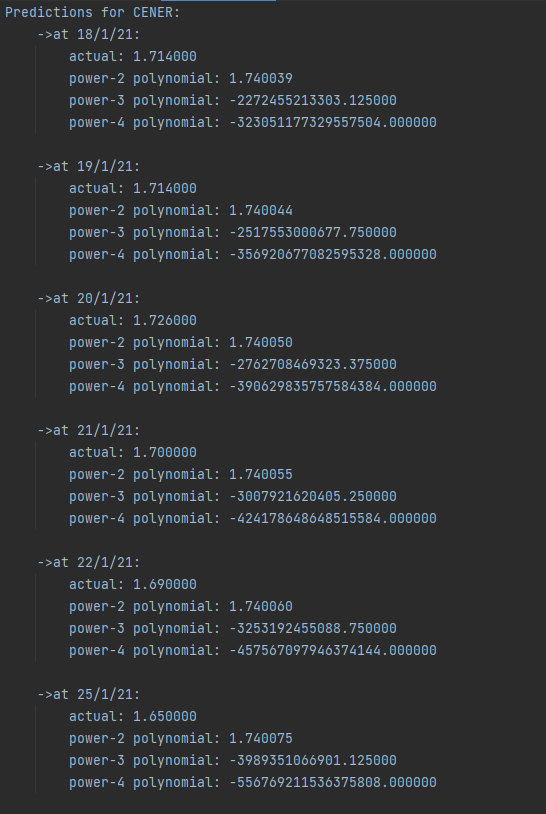
\includegraphics[scale=0.7]{images/cener_future.png}
    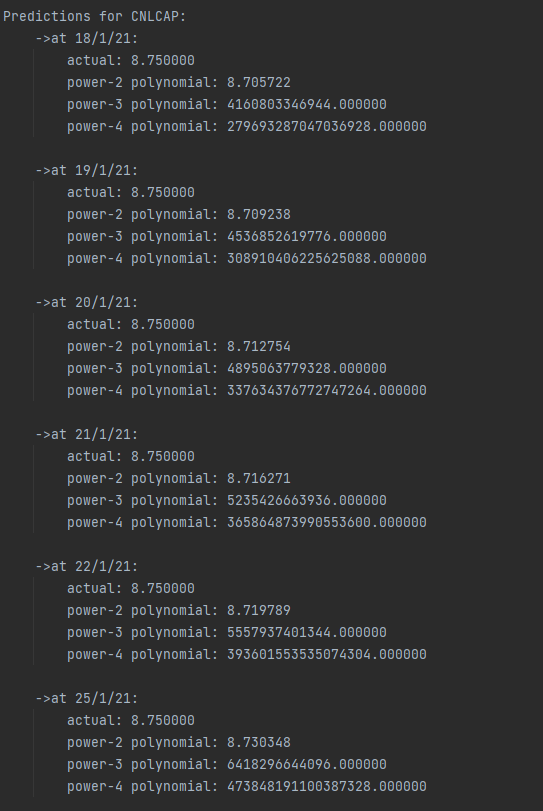
\includegraphics[scale=0.7]{images/cnlcap_future.png}
\end{center}
\gt Παρατηρούμε ότι το πολυώνυμο 2ου βαθμού δίνει μια ικανοποιητική
\gt(για ελάχιστα τετράγωνα) προσέγγιση της πραγματικής τιμής για κάθε συνεδρίαση, ενώ
\gtτα πολυώνυμα 3ου και 4ου βαθμού εξωστρακίζονται πλήρως, επιστρέφοντας παράλογα
\gtνούμερα με εξωφρενικά σφάλματα.

\gtΤο ίδιο συμβαίνει και για τις τιμές των συνεδριάσεων
\gtπου χρησιμοποιήσαμε για να χτίσουμε τα πολυώνυμα των ελάχιστων τετραγώνων:
\begin{center}
    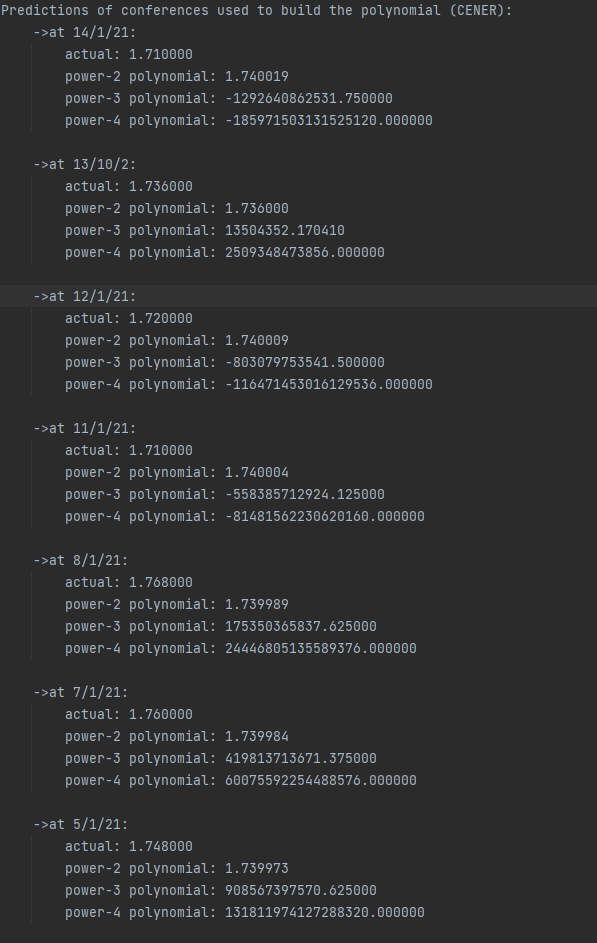
\includegraphics[scale=0.7]{images/cener_past.png}
    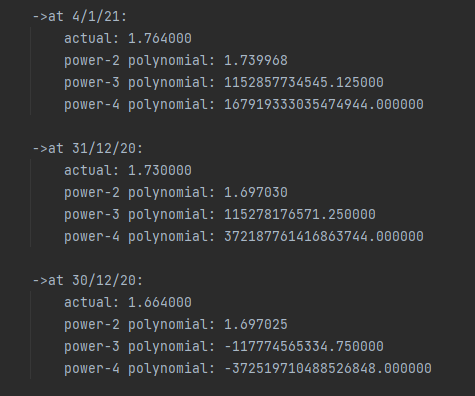
\includegraphics[scale=0.7]{images/cener_past1.png}
    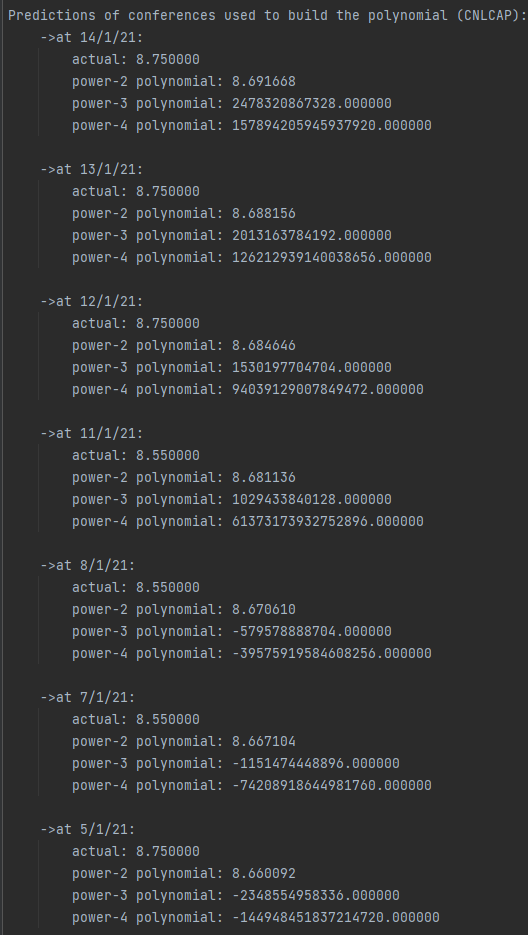
\includegraphics[scale=0.7]{images/cnlcap_past.png}
    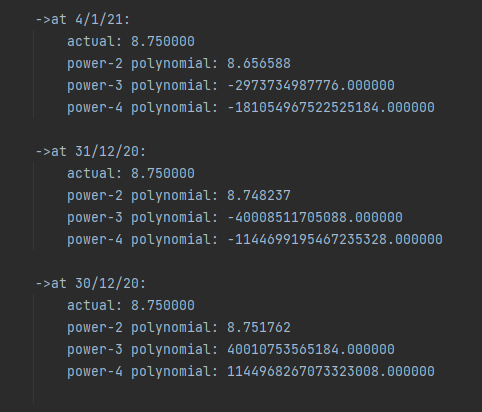
\includegraphics[scale=0.7]{images/cnlcap_past1.png}
\end{center}

\gt Καταλήγουμε πως σε περίπτωση που χρειάζεται να προβλέψουμε αυξομειούμενη,
\lt volatile \gt τιμή, όπως αυτές του χρηματιστηρίου ή των κρυπτονομισμάτων,
\gt είναι καλύτερο να καταφεύγουμε σε ελάχιστα τετράγωνα βαθμού 2.
%%------------EOF------------%%
\end{document}